%%%%%%%%%%%%%%%%%%%%%%%%%%%%%%%%%%%%%%%%%%%%%%%%%%%%%%%%%%%%%%%%%%%%%%%%
\chapter{Expert Opinion Elicitation for Assisting Lesion Image Classifier With Patient Data}\label{chap:Elicitation}\chaptermark{Expert Opinion Elicitation}
%%%%%%%%%%%%%%%%%%%%%%%%%%%%%%%%%%%%%%%%%%%%%%%%%%%%%%%%%%%%%%%%%%%%%%%%

\begin{center}
	\begin{minipage}{0.8\textwidth}
		\begin{small}
			This chapter addresses research question \ref{question2}, presents our questionnaire based expert opinion elicitation method for calculating disease probability from patient data and an approach for combining independent probability estimates from multiple modalities. Contents from this chapter have been used in the following article:
			\begin{itemize}
				\item \fullcite{Hossain2022Elicitation}
			\end{itemize}  
		\end{small}
	\end{minipage}
	\vspace{0.5cm}
\end{center}

\minitoc

%%%%%%%%%%%%%%%%%%%%%%%%%%%%%%%%%%%%%%%%%%%%%%%%%%%%%%%%%%%%%%%%%%%%%%%%
\section{Introduction}
%%%%%%%%%%%%%%%%%%%%%%%%%%%%%%%%%%%%%%%%%%%%%%%%%%%%%%%%%%%%%%%%%%%%%%%%
When the dermatologists rechecked the annotations of the Lyme image dataset misclassified by most of the convolutional neural networks (CNNs) (discussed in Chapter \ref{chap:Pretraining}) they found mistakes in some of the initial annotations. This suggests that some images are too confusing to classify even for the experts without additional context from patient data.

Expert opinion elicitation can be effective when high quality data is difficult to collect \cite{Wilson2018}. Point estimates (such as medians or means), intervals of uncertainty (such as confidence intervals or quartiles), or probability distributions can all be included in the measurements elicited \cite{cadham2022use}. Expert opinion elicitation and aggregation processes can be classified into two categories: behavioral and mathematical approaches \cite{Clemen1999, cadham2022use}. The behavioral approach tries to produce group consensus among experts whereas, the mathematical approach combines subjective probabilities from experts using mathematical methods (some form of averaging) \cite{cadham2022use}.

Expert elicitation proved effective for medical diagnosis and decision making. For example, Van Der Gaag et al. \cite{VanDerGaag2002} created a probabilistic network to describe the oesophageal cancer presentation characteristics and the pathophysiological mechanisms of invasion and metastasis by eliciting opinions from two experts. Saegerman et al. \cite{Saegerman2022} elicited opinions from eleven European experts to rank the drivers of the emergence of bovine besnoitiosis a chronic disease in cattle.  Wilson et al. \cite{Wilson2018} elicited opinions from sixteen experts on the disease progression probability in patients with untreated melanoma. The article by Cadham et al. \cite{cadham2022use} contains a detailed review of the application of expert elicitation in health research computational modeling studies.

In our study, for the first time, we elicited opinions from fifteen expert dermatologists to create a model for calculating erythema migrans (EM) probability from patient data as an early symptom of Lyme disease. First, with the help of the experts, a questionnaire was prepared based on questions that the doctors ask during EM diagnosis. The traditional expert elicitation process of collecting probability estimates for cases based on the questionnaire is time consuming and it is difficult for doctors to provide probability estimates for cases or distribution parameters. Therefore, we opted for a more relaxed approach of relative weight assignment to different answers to the questions and converted the doctor’s evaluations to EM probabilities utilizing Gaussian mixture model (GMM) based density estimation (described in Section \ref{sec:GMM}). To validate the elicited probability model and explain its behavior to the experts we utilized formal concept analysis (described in Section \ref{sec:FCA}) and decision tree (described in Section \ref{sec:DecTree}). The elicited patient data based EM probability model will be useful for assisting image-based EM classifiers with additional context from patient data. We also proposed an algorithm for combining the EM probability score from a deep learning image classifier with the elicited probability score from patient data. The proposed algorithm ensures veto power for the patient data. The elicited probability score and the proposed algorithm can be utilized to make image based deep learning Lyme disease pre-scanners robust and the techniques will be useful for questionnaire based opinion elicitation of other diseases.

The rest of the chapter is structured as follows: Section \ref{sec:elicitation} describes the expert elicitation process and elicitation result; Section \ref{sec:combining_prob} contains the strategy for combining probabilities; finally, Section \ref{sec:elicitation_conclusion} provides concluding remarks.

\section{Elicitation Method}\label{sec:elicitation}
The details of our expert elicitation process like expert recruitment, questionnaire preparation, experts’ opinion collection, elicitation methods, result, and analysis are presented in the following subsections.

\subsection{Expert Selection}
The recruited experts are hospital practitioners who are infectious disease specialists or dermatologists working in reference centers for tick-borne diseases of France - Centres de Référence des Maladies Vectorielles liées aux Tiques (CRMVT) \cite{CRMVTRef}. At a CRMVT steering committee meeting held in June 2021 with participants from all the reference centers, Professor Olivier Lesens (Infectious and Tropical Diseases Department, CRIOA, CHU Clermont-Ferrand, France) explained the importance of expert elicitation for calculating EM probability based on patient data and requested the interested experts to participate in the elicitation process. Fifteen experts agreed to participate\footnote{The experts did not receive any monetary benefits for participating in the elicitation process.}. Table \ref{tab:expert_table} lists the reference centers and the corresponding number of experts participating in the elicitation process.
\begin{table}[tb!]
	\caption{Experts recruited for erythema migrans probability elicitation.}
	\label{tab:expert_table}
	\resizebox{\textwidth}{!}{%
		\begin{tabular}{lc}
			\toprule
			\multicolumn{1}{c}{\textbf{Center}} &
			\textbf{Number of Participating Experts} \\ \midrule
			\begin{tabular}[c]{l}\textbf{CRMVT du Grand Ouest}\\ Hôpital Pontchaillou  \\ Centre Urgences-Réanimations \\ 2 rue Henri Le Guilloux \\ 35033 Rennes Cedex 09\end{tabular} &
			2 \\ \cmidrule(lr){1-2}
			\begin{tabular}[c]{l}\textbf{CRMVT Ile-de-France et Hauts-de-France} \\ Hôpital de Villeneuve-Saint-Georges \\ Secrétariat du centre Lyme \\ 40 allée de la Source \\ 94195 Villeneuve-Saint-Georges Cedex\end{tabular} &
			2 \\ \cmidrule(lr){1-2}
			\begin{tabular}[c]{l}\textbf{CRMVT de Strasbourg} \\ Nouvel Hôpital Civil - Hôpitaux Universitaires de Strasbourg (HUS) \\ 1 place de l'Hôpital BP461 \\ 67091 STRASBOURG Cedex\end{tabular} &
			1 \\ \cmidrule(lr){1-2}
			\begin{tabular}[c]{l}\textbf{CRMVT de Nancy} \\ Centre Hospitalier Régional et Universitaire \\ (CHRU) de Nancy \\ Rue du Morvan \\ 54500 Vandœuvre-lès-Nancy\end{tabular} &
			1 \\ \cmidrule(lr){1-2}
			\begin{tabular}[c]{l}\textbf{CRMVT de Clermont-Ferrand} \\ Service des Maladies Infectieuses et Tropicales \\ CHU Gabriel Montpied \\ 58, Rue Montalembert \\ 63003 Clermont-Ferrand Cedex 1\end{tabular} &
			8 \\ \cmidrule(lr){1-2}
			\begin{tabular}[c]{l}\textbf{CRMVT de Saint-Etienne} \\ Service des Maladies Infectieuses et Tropicales Hôpital Nord \\ Avenue Albert Raimond \\ 42270 Saint-Priest-en-Jarez\end{tabular} &
			1 \\ \bottomrule
		\end{tabular}%
	}
\end{table}

\subsection{Questionnaire and Experts’ Evaluation}
For the EM probability elicitation, a questionnaire was prepared based on questions about the context of onset and progression of the skin lesion that a physician usually asks when diagnosing EM. The questionnaire is based on a previous study concerning the collection of EM related data from rural areas of France \cite{Letertre-Gibert2020}. The questionnaire was finalized through several meetings held in April 2020 among the doctors of CRMVT in Clermont-Ferrand and experts in tick ecology from the French national research institute for agriculture, food and the environment - \selectlanguage{french}Institut national de recherche pour l'agriculture, l'alimentation et l'environnement (INRAE) \selectlanguage{english}\cite{INRAE}. Experts who volunteered to participate in the elicitation process at the meeting in June 2021 agreed that there were many possible cases from the combination of the questions and answers, and it was time consuming and difficult for them to provide probability estimates for all those different cases. Therefore, experts agreed to independently assign relative weights to different possible answers associated with each question. The assigned weight values are in the range $-1$ to $+3$ (a higher value represents a higher contribution of the answer towards the possibility of the EM). The experts were contacted via email with detailed instructions to provide their weight attributions independently. Table \ref{tab:initial_opinion} lists the questions, answers, and weight attribution from the doctors.
\begin{table}[tb!]
	\caption[Questionnaire and doctors’ weight attribution for erythema migrans]{Questionnaire and doctors’ weight attribution for erythema migrans. The assigned weight values are in the range $-1$ to $+3$ (a higher value represents a higher contribution of the answer towards the possibility of the erythema migrans). $d_{1}$ to $d_{15}$ represents the doctors.}
	\label{tab:initial_opinion}
	\resizebox{\textwidth}{!}{%
		\begin{tabular}{cllcccccccccccccccc}
			\toprule
			\multirow{2}{*}{\textbf{Question}} &
			\multicolumn{2}{c}{\multirow{2}{*}{\textbf{Answer}}} &
			\multicolumn{16}{c}{\textbf{\begin{tabular}[c]{@{}c@{}}Weight Assigned by Doctors \\ (Doctor's Evaluation)\end{tabular}}} \\ \cmidrule(l){4-19} 
			&
			\multicolumn{2}{c}{} &
			$d_{1}$ &
			$d_{2}$ &
			$d_{3}$ &
			$d_{4}$ &
			$d_{5}$ &
			$d_{6}$ &
			$d_{7}$ &
			$d_{8}$ &
			$d_{9}$ &
			$d_{10}$ &
			$d_{11}$ &
			$d_{12}$ &
			$d_{13}$ &
			$d_{14}$ &
			$d_{15}$ &
			Average \\ \midrule \addlinespace[2pt]
			\multirow{7}{*}[-2.7em]{\begin{tabular}[c]{@{}c@{}}Other symptoms observed \\ alongside the skin lesion\end{tabular}} &
			\multicolumn{2}{l}{No} &
			0 &
			0 &
			3 &
			0 &
			0 &
			1 &
			2 &
			1 &
			2 &
			1 &
			2 &
			1 &
			1 &
			2 &
			3 &
			1.27 \\ \addlinespace[2pt] \cmidrule(lr) {2-19} \addlinespace[2pt]
			&
			\multicolumn{2}{l}{Fever} &
			-1 &0 &-1 &1 &1 &1 &1 &1 &1 &1 &1 &1 &1 &1 &0 &0.6 \\ \addlinespace[2pt] \cmidrule(lr){2-19} \addlinespace[2pt]
			&
			\multicolumn{2}{l}{Fatigue} &
			0 &1 &1 &2 &0 &0 &1 &1 &1 &1 &1 &0 &1 &0 &0 &0.67 \\ \addlinespace[2pt] \cmidrule(lr){2-19} \addlinespace[2pt]
			&
			\multicolumn{2}{l}{Faintness} &
			0 &0 &1 &0 &0 &0 &0 &0 &1 &0 &1 &-1 &1 &0 &0 &0.2 \\ \addlinespace[2pt] \cmidrule(lr){2-19} \addlinespace[2pt]
			&
			\multicolumn{2}{l}{Joint pain} &
			0 &0 &-1 &0 &2 &0 &1 &1 &0 &2 &1 &1 &1 &0 &0 &0.53 \\ \addlinespace[2pt] \cmidrule(lr){2-19} \addlinespace[2pt]
			&
			\multicolumn{2}{l}{Headache} &
			1 &
			1 &
			-1 &
			2 &
			2 &
			1 &
			1 &
			1 &
			1 &
			1 &
			1 &
			1 &
			1 &
			0 &
			0 &
			0.87 \\ \addlinespace[2pt] \cmidrule(lr){2-19} \addlinespace[2pt]
			&
			\multicolumn{2}{l}{Itching} &
			-1 &
			-1 &
			-1 &
			-1 &
			1 &
			-1 &
			0 &
			0 &
			0 &
			1 &
			-0.5 &
			-1 &
			-1 &
			1 &
			0 &
			-0.3 \\ \addlinespace[2pt] \cmidrule(lr){1-19} \addlinespace[2pt]
			\multirow{4}{*}[-1.5em]{\begin{tabular}[c]{@{}c@{}}What was the maximum \\ size of the red rash\end{tabular}} &
			\multicolumn{2}{l}{$<1$ cm} &
			-1 &
			-1 &
			0 &
			-1 &
			-1 &
			-1 &
			-1 &
			0 &
			0 &
			-1 &
			-1 &
			-1 &
			-1 &
			1 &
			-1 &
			-0.67 \\ \addlinespace[2pt] \cmidrule(lr){2-19} \addlinespace[2pt]
			&
			\multicolumn{2}{l}{1 to 5 cm} &
			1 &
			1 &
			1 &
			0 &
			1 &
			0 &
			1 &
			1 &
			2 &
			1 &
			1 &
			1 &
			1 &
			2 &
			1 &
			1 \\ \addlinespace[2pt] \cmidrule(lr){2-19} \addlinespace[2pt]
			&
			\multicolumn{2}{l}{$>5$ cm} &
			3 &
			2 &
			2 &
			2 &
			3 &
			2 &
			3 &
			2 &
			1 &
			3 &
			2 &
			2 &
			3 &
			3 &
			3 &
			2.4 \\ \addlinespace[2pt] \cmidrule(lr){2-19} \addlinespace[2pt]
			&
			\multicolumn{2}{l}{I do not know} &
			0 &
			0 &
			0 &
			0 &
			0 &
			0 &
			-1 &
			1 &
			0 &
			0 &
			0 &
			0 &
			0 &
			0 &
			0 &
			0 \\ \addlinespace[2pt] \cmidrule(lr){1-19} \addlinespace[2pt]
			\multirow{3}{*}[-1em]{\begin{tabular}[c]{@{}c@{}}Is the size of the red rash \\ increasing or has it \\ gradually increased\end{tabular}} &
			\multicolumn{2}{l}{Yes} &
			3 &
			1 &
			3 &
			3 &
			3 &
			3 &
			3 &
			3 &
			2 &
			3 &
			3 &
			3 &
			3 &
			3 &
			3 &
			2.8 \\ \addlinespace[2pt] \cmidrule(lr){2-19} \addlinespace[2pt]
			&
			\multicolumn{2}{l}{No} &
			0 &
			-1 &
			-1 &
			-1 &
			-1 &
			-1 &
			-1 &
			0 &
			-1 &
			0 &
			-1 &
			-1 &
			-1 &
			1 &
			-1 &
			-0.67 \\ \addlinespace[2pt] \cmidrule(lr){2-19} \addlinespace[2pt]
			&
			\multicolumn{2}{l}{I do not know} &
			0 &
			0 &
			0 &
			0 &
			0 &
			0 &
			0 &
			1 &
			0 &
			0 &
			0 &
			0 &
			0 &
			0 &
			0 &
			0.07 \\ \addlinespace[2pt] \cmidrule(lr){1-19} \addlinespace[2pt]
			\multirow{2}{*}{\begin{tabular}[c]{@{}c@{}}Have you seen a tick bite \\on this red rash \\in the past 30 days\end{tabular}} &
			\multicolumn{2}{l}{Yes} &
			3 &
			2 &
			3 &
			2 &
			3 &
			1 &
			3 &
			3 &
			2 &
			3 &
			2 &
			3 &
			1 &
			3 &
			3 &
			2.47 \\ \addlinespace[4pt] \cmidrule(lr){2-19} \addlinespace[2pt]
			&
			\multicolumn{2}{l}{No} &
			0 &
			0 &
			0 &
			0 &
			0 &
			1 &
			0 &
			1 &
			0 &
			0 &
			-0.5 &
			-1 &
			0 &
			1 &
			0 &
			0.1 \\ \addlinespace[2pt] \cmidrule(lr){1-19} \addlinespace[2pt]
			\multirow{4}{*}[-1.5em]{\begin{tabular}[c]{@{}c@{}}Frequency of tick bites \\in the last 30 days \\before the appearance \\ of the red rash\end{tabular}} &
			\multicolumn{2}{l}{Never} &
			-1 &
			-1 &
			0 &
			0 &
			-1 &
			0 &
			0 &
			0 &
			0 &
			0 &
			-1 &
			-1 &
			0 &
			-1 &
			0 &
			-0.4 \\ \addlinespace[2pt] \cmidrule(lr){2-19} \addlinespace[2pt]
			&
			\multicolumn{2}{l}{1 time} &
			0 &
			0 &
			2 &
			1 &
			1 &
			1 &
			1 &
			1 &
			2 &
			1 &
			1 &
			1 &
			1 &
			2 &
			1 &
			1.07 \\ \addlinespace[2pt] \cmidrule(lr){2-19} \addlinespace[2pt]
			&
			\multicolumn{2}{l}{2 to 5 times} &
			1 &
			1 &
			3 &
			1 &
			1 &
			1 &
			1 &
			2 &
			2 &
			1 &
			2 &
			1 &
			1 &
			3 &
			1 &
			1.47 \\ \addlinespace[2pt] \cmidrule(lr){2-19} \addlinespace[2pt]
			&
			\multicolumn{2}{l}{$>5$ times} &
			2 &
			2 &
			1 &
			2 &
			2 &
			1 &
			1 &
			2 &
			2 &
			2 &
			3 &
			1 &
			1 &
			3 &
			2 &
			1.8 \\ \addlinespace[2pt] \cmidrule(lr){1-19} \addlinespace[2pt]
			\multirow{2}{*}{\begin{tabular}[c]{@{}c@{}}Outdoor activities in the \\last  30 days before the \\onset of the red rash\end{tabular}} &
			\multicolumn{2}{l}{Yes} &
			1 &
			1 &
			2 &
			2 &
			1 &
			1 &
			2 &
			2 &
			2 &
			2 &
			2 &
			2 &
			1 &
			3 &
			2 &
			1.73 \\ \addlinespace[2pt] \cmidrule(lr){2-19} \addlinespace[2pt]
			&
			\multicolumn{2}{l}{No} &
			-1 &
			-1 &
			-1 &
			-1 &
			-1 &
			0 &
			-1 &
			1 &
			-1 &
			-1 &
			-1 &
			-1 &
			0 &
			-1 &
			0 &
			-0.67 \\\addlinespace[5pt] \bottomrule
		\end{tabular}%
	}
\end{table}
After receiving the weight attributions from all the experts, they participated in a meeting in November 2021 and agreed that fever, fatigue, faintness, and headache should contribute equally if one or more of these answers were present and the contribution should be the average of these four answers. Therefore, the four answers were replaced with one, and the possible cases reduced to 1,536 from 12,288 cases. This modification is shown in Table \ref{tab:modified_opinion}.
\begin{table}[tb!]
	\caption[Weight modified questionnaire and doctors’ weight attribution for erythema migrans]{Weight modified questionnaire and doctors’ weight attribution for erythema migrans. The assigned weight values are in the range $-1$ to $+3$ (a higher value represents a higher contribution of the answer towards the possibility of the erythema migrans). $d_{1}$ to $d_{15}$ represents the doctors.}
	\label{tab:modified_opinion}
	\resizebox{\textwidth}{!}{%
		\begin{tabular}{cllcccccccccccccccc}
			\toprule
			\multirow{2}{*}{\textbf{Question}} &
			\multicolumn{2}{c}{\multirow{2}{*}{\textbf{Answer}}} &
			\multicolumn{16}{c}{\textbf{\begin{tabular}[c]{@{}c@{}}Weight Assigned by Doctors \\ (Doctor's Evaluation)\end{tabular}}} \\ \cmidrule(l){4-19} 
			&
			\multicolumn{2}{c}{} &
			$d_{1}$ &
			$d_{2}$ &
			$d_{3}$ &
			$d_{4}$ &
			$d_{5}$ &
			$d_{6}$ &
			$d_{7}$ &
			$d_{8}$ &
			$d_{9}$ &
			$d_{10}$ &
			$d_{11}$ &
			$d_{12}$ &
			$d_{13}$ &
			$d_{14}$ &
			$d_{15}$ &
			Average \\ \midrule \addlinespace[2pt]
			\multirow{4}{*}[-2.7em]{\begin{tabular}[c]{@{}c@{}}Other symptoms observed \\ alongside the skin lesion $(q_{1})$\end{tabular}} &
			\multicolumn{2}{l}{No $(a_{1,q_{1}})$} &
			0 &
			0 &
			3 &
			0 &
			0 &
			1 &
			2 &
			1 &
			2 &
			1 &
			2 &
			1 &
			1 &
			2 &
			3 &
			1.27 \\ \addlinespace[2pt] \cmidrule(lr) {2-19} \addlinespace[2pt]
			&
			\multicolumn{2}{l}{\begin{tabular}[c]{@{}l@{}}Fever/\\ Fatigue/\\ Faintness/\\ Headache $(a_{2,q_{1}})$\end{tabular}} &
			\rotatebox[origin=c]{90}{-0.25} &
			\rotatebox[origin=c]{90}{0.25} &
			\rotatebox[origin=c]{90}{0} &
			\rotatebox[origin=c]{90}{0.75} &
			\rotatebox[origin=c]{90}{0.75} &
			\rotatebox[origin=c]{90}{0.25} &
			\rotatebox[origin=c]{90}{0.75} &
			\rotatebox[origin=c]{90}{0.75} &
			\rotatebox[origin=c]{90}{0.75} &
			\rotatebox[origin=c]{90}{1} &
			\rotatebox[origin=c]{90}{1} &
			\rotatebox[origin=c]{90}{0.25} &
			\rotatebox[origin=c]{90}{1} &
			\rotatebox[origin=c]{90}{0.25} &
			\rotatebox[origin=c]{90}{0} &
			\rotatebox[origin=c]{90}{0.5} \\ \addlinespace[2pt] \cmidrule(lr){2-19} \addlinespace[2pt]
			&
			\multicolumn{2}{l}{Joint pain $(a_{3,q_{1}})$} &
			1 &
			1 &
			-1 &
			2 &
			2 &
			1 &
			1 &
			1 &
			1 &
			1 &
			1 &
			1 &
			1 &
			0 &
			0 &
			0.87 \\ \addlinespace[2pt] \cmidrule(lr){2-19} \addlinespace[2pt]
			&
			\multicolumn{2}{l}{Itching $(a_{4,q_{1}})$} &
			-1 &
			-1 &
			-1 &
			-1 &
			1 &
			-1 &
			0 &
			0 &
			0 &
			1 &
			-0.5 &
			-1 &
			-1 &
			1 &
			0 &
			-0.3 \\ \addlinespace[2pt] \cmidrule(lr){1-19} \addlinespace[2pt]
			\multirow{4}{*}[-1.5em]{\begin{tabular}[c]{@{}c@{}}What was the maximum \\ size of the red rash $(q_{2})$\end{tabular}} &
			\multicolumn{2}{l}{$<1$ cm $(a_{1,q_{2}})$} &
			-1 &
			-1 &
			0 &
			-1 &
			-1 &
			-1 &
			-1 &
			0 &
			0 &
			-1 &
			-1 &
			-1 &
			-1 &
			1 &
			-1 &
			-0.67 \\ \addlinespace[2pt] \cmidrule(lr){2-19} \addlinespace[2pt]
			&
			\multicolumn{2}{l}{1 to 5 cm $(a_{2,q_{2}})$} &
			1 &
			1 &
			1 &
			0 &
			1 &
			0 &
			1 &
			1 &
			2 &
			1 &
			1 &
			1 &
			1 &
			2 &
			1 &
			1 \\ \addlinespace[2pt] \cmidrule(lr){2-19} \addlinespace[2pt]
			&
			\multicolumn{2}{l}{$>5$ cm $(a_{3,q_{2}})$} &
			3 &
			2 &
			2 &
			2 &
			3 &
			2 &
			3 &
			2 &
			1 &
			3 &
			2 &
			2 &
			3 &
			3 &
			3 &
			2.4 \\ \addlinespace[2pt] \cmidrule(lr){2-19} \addlinespace[2pt]
			&
			\multicolumn{2}{l}{I do not know $(a_{4,q_{2}})$} &
			0 &
			0 &
			0 &
			0 &
			0 &
			0 &
			-1 &
			1 &
			0 &
			0 &
			0 &
			0 &
			0 &
			0 &
			0 &
			0 \\ \addlinespace[2pt] \cmidrule(lr){1-19} \addlinespace[2pt]
			\multirow{3}{*}[-1em]{\begin{tabular}[c]{@{}c@{}}Is the size of the red rash \\ increasing or has it \\ gradually increased  $(q_{3})$\end{tabular}} &
			\multicolumn{2}{l}{Yes $(a_{1,q_{3}})$} &
			3 &
			1 &
			3 &
			3 &
			3 &
			3 &
			3 &
			3 &
			2 &
			3 &
			3 &
			3 &
			3 &
			3 &
			3 &
			2.8 \\ \addlinespace[2pt] \cmidrule(lr){2-19} \addlinespace[2pt]
			&
			\multicolumn{2}{l}{No $(a_{2,q_{3}})$} &
			0 &
			-1 &
			-1 &
			-1 &
			-1 &
			-1 &
			-1 &
			0 &
			-1 &
			0 &
			-1 &
			-1 &
			-1 &
			1 &
			-1 &
			-0.67 \\ \addlinespace[2pt] \cmidrule(lr){2-19} \addlinespace[2pt]
			&
			\multicolumn{2}{l}{I do not know $(a_{3,q_{3}})$} &
			0 &
			0 &
			0 &
			0 &
			0 &
			0 &
			0 &
			1 &
			0 &
			0 &
			0 &
			0 &
			0 &
			0 &
			0 &
			0.07 \\ \addlinespace[2pt] \cmidrule(lr){1-19} \addlinespace[2pt]
			\multirow{2}{*}{\begin{tabular}[c]{@{}c@{}}Have you seen a tick bite \\on this red rash \\in the past 30 days $(q_{4})$\end{tabular}} &
			\multicolumn{2}{l}{Yes $(a_{1,q_{4}})$} &
			3 &
			2 &
			3 &
			2 &
			3 &
			1 &
			3 &
			3 &
			2 &
			3 &
			2 &
			3 &
			1 &
			3 &
			3 &
			2.47 \\ \addlinespace[4pt] \cmidrule(lr){2-19} \addlinespace[2pt]
			&
			\multicolumn{2}{l}{No $(a_{2,q_{4}})$} &
			0 &
			0 &
			0 &
			0 &
			0 &
			1 &
			0 &
			1 &
			0 &
			0 &
			-0.5 &
			-1 &
			0 &
			1 &
			0 &
			0.1 \\ \addlinespace[2pt] \cmidrule(lr){1-19} \addlinespace[2pt]
			\multirow{4}{*}[-1.5em]{\begin{tabular}[c]{@{}c@{}}Frequency of tick bites \\in the last 30 days \\before the appearance \\ of the red rash $(q_{5})$\end{tabular}} &
			\multicolumn{2}{l}{Never $(a_{1,q_{5}})$} &
			-1 &
			-1 &
			0 &
			0 &
			-1 &
			0 &
			0 &
			0 &
			0 &
			0 &
			-1 &
			-1 &
			0 &
			-1 &
			0 &
			-0.4 \\ \addlinespace[2pt] \cmidrule(lr){2-19} \addlinespace[2pt]
			&
			\multicolumn{2}{l}{1 time $(a_{2,q_{5}})$} &
			0 &
			0 &
			2 &
			1 &
			1 &
			1 &
			1 &
			1 &
			2 &
			1 &
			1 &
			1 &
			1 &
			2 &
			1 &
			1.07 \\ \addlinespace[2pt] \cmidrule(lr){2-19} \addlinespace[2pt]
			&
			\multicolumn{2}{l}{2 to 5 times $(a_{3,q_{5}})$} &
			1 &
			1 &
			3 &
			1 &
			1 &
			1 &
			1 &
			2 &
			2 &
			1 &
			2 &
			1 &
			1 &
			3 &
			1 &
			1.47 \\ \addlinespace[2pt] \cmidrule(lr){2-19} \addlinespace[2pt]
			&
			\multicolumn{2}{l}{$>5$ times $(a_{4,q_{5}})$} &
			2 &
			2 &
			1 &
			2 &
			2 &
			1 &
			1 &
			2 &
			2 &
			2 &
			3 &
			1 &
			1 &
			3 &
			2 &
			1.8 \\ \addlinespace[2pt] \cmidrule(lr){1-19} \addlinespace[2pt]
			\multirow{2}{*}{\begin{tabular}[c]{@{}c@{}}Outdoor activities in the \\last  30 days before the \\onset of the red rash  $(q_{6})$\end{tabular}} &
			\multicolumn{2}{l}{Yes $(a_{1,q_{6}})$} &
			1 &
			1 &
			2 &
			2 &
			1 &
			1 &
			2 &
			2 &
			2 &
			2 &
			2 &
			2 &
			1 &
			3 &
			2 &
			1.73 \\ \addlinespace[2pt] \cmidrule(lr){2-19} \addlinespace[2pt]
			&
			\multicolumn{2}{l}{No $(a_{2,q_{6}})$} &
			-1 &
			-1 &
			-1 &
			-1 &
			-1 &
			0 &
			-1 &
			1 &
			-1 &
			-1 &
			-1 &
			-1 &
			0 &
			-1 &
			0 &
			-0.67 \\\addlinespace[5pt] \bottomrule
		\end{tabular}%
	}
\end{table}

\subsection{Opinion Elicitation}
Following are some notations used in the rest of the manuscript:
\begin{itemize}
	
	\item Set of doctors, \( D = \{ d_{e}\vert e = 1,\ldots ,n_e\}\).
	
	\item Set of questions, \( Q = \{ q_{i}\vert i = 1,\ldots ,n_i\}\).
	
	\item Set of possible cases, \( C = \{ c_{l}\vert l = 1,\ldots ,n_l\}\).
	
	\item Total number of answers corresponding to $q_{i} $ question $=$  $n_{q_{i}}$. \\For example, $n_{q_{2}}=4$ because question $q_{2}$ has four possible answers (refer to Table \ref{tab:modified_opinion}).
%	\vfill
	\item $j^{th}$ answer corresponding to $q_{i}$ question,\begin{displaymath}
		a_{j,q_{i}}= 
		\begin{cases}
			1,& \text{if the answer is true } \\
			0,              & \text{otherwise}
		\end{cases}, \text{where} \, j = 1,\ldots , n_{q_{i}}
	\end{displaymath}
	
	\item Weight assigned by doctor $d_{e}$ to $a_{j,q_{i}}$ answer $=  w_{d_{e},a_{j,q_{i}}}$. \\For example, $ w_{d_{1},a_{3,q_{2}}}=3$ because the third answer to second question has a weight of 3 assigned by the first doctor (refer to Table \ref{tab:modified_opinion}).
	
\end{itemize}

Our opinion elicitation task for Lyme disease involved fifteen experts, the prepared questionnaire contains six questions and the possible cases from the combination of questions and answers is 1,536. So, for the Lyme disease task  $n_e=15,\, n_i=6,\,\text{and}\,n_l=1536$. First, we summarized each of the $n_l$ possible cases as a weight sum $s_{c_{l}}$ as shown in Equation (\ref{eq:weight-sum}).
\begin{equation}\label{eq:weight-sum}
	s_{c_{l}} = \sum_{i = 1}^{\vert Q\vert }\sum_{j = 1}^{n_{q_{i}}}a_{j,q_{i}}\times\left(\frac{1}{\vert D\vert }\sum_{d = 1}^{\vert D\vert }w_{d_{e},a_{j,q_{i}}}\right)
\end{equation}
The set of case weight sum is defined as \( S = \{s_{c_{l}}\vert l = 1,\ldots ,n_l\}\). Then, we normalized each case weight sum with min-max normalization as shown in Equation (\ref{eq:weight-sum-norm}).
\begin{equation}\label{eq:weight-sum-norm}
	\tilde{s}_{c_l}=\frac{s_{c_l}-\min (S)}{\max (S)-\min (S)}
\end{equation}
The set of min-max normalized case weight sum is defined as \(\tilde{S} = \{\tilde{s}_{c_{l}}\vert l = 1,\ldots ,n_l\}\). We proposed three approaches to the experts to convert the normalized case weight sum to a probability score for EM. The following subsections explain the three approaches.

\subsubsection{Cumulative Probability from Density Estimate Based on GMM}
\label{sec:GMM-approach}
We modeled our normalized weight sum data density using a GMM with two components. The number of components was selected based on the intuition that there are two sub populations within the data: one is the ill sub population and the other one is not ill sub population. The number of components was also supported by AIC and BIC values. Table \ref{tab:GMM_params} lists the selected parameters for the GMM. 
\begin{table}[htb!]
	\centering
	\caption[Parameters of Gaussian mixture model used to model the density of min-max normalized weight sum of erythema migrans cases]{Parameters of Gaussian mixture model used to model the density of min-max normalized weight sum of erythema migrans cases. $\varnothing$ , $\mu$ ,and $\sigma$ represent mixture weight, mean and standard deviation respectively.}
	\label{tab:GMM_params}
	\begin{tabular}{cc}
		\toprule
		\multicolumn{1}{c}{\textbf{Parameter Name}} & \textbf{Value} \\ \midrule
		Components                                  & 2              \\
		$\varnothing_{1} $                            & 0.364801       \\
		$\varnothing_{2} $                            & 0.635199       \\
		$\mu_{1}  $                                   & 0.359548       \\
		$\mu_{2} $                                    & 0.572878       \\
		$\sigma_{1} $                                 & 0.128782       \\
		$\sigma_{2}$                                  & 0.156241       \\ \bottomrule
	\end{tabular}
\end{table}
The blue curve in Figure \ref{fig:elicitation_approaches} shows the estimated density function using GMM. We defined the cumulative probability \cite{Carr2003} of a normalized case weight sum from the GMM density estimate as the probability of EM as shown in Equation (\ref{eq:GMM}).
\begin{equation}
	\label{eq:GMM}
	\hat{F}_{GMM}\left(x\right) =  \int_{-\infty }^{x}\left(\sum_{m = 1}^{2}\varnothing_{m}\mathcal{N}\left(x\right\vert  \mu_{m},\sigma_{m})\right)dx
\end{equation}
\begin{figure}[htb!]
	\centering
	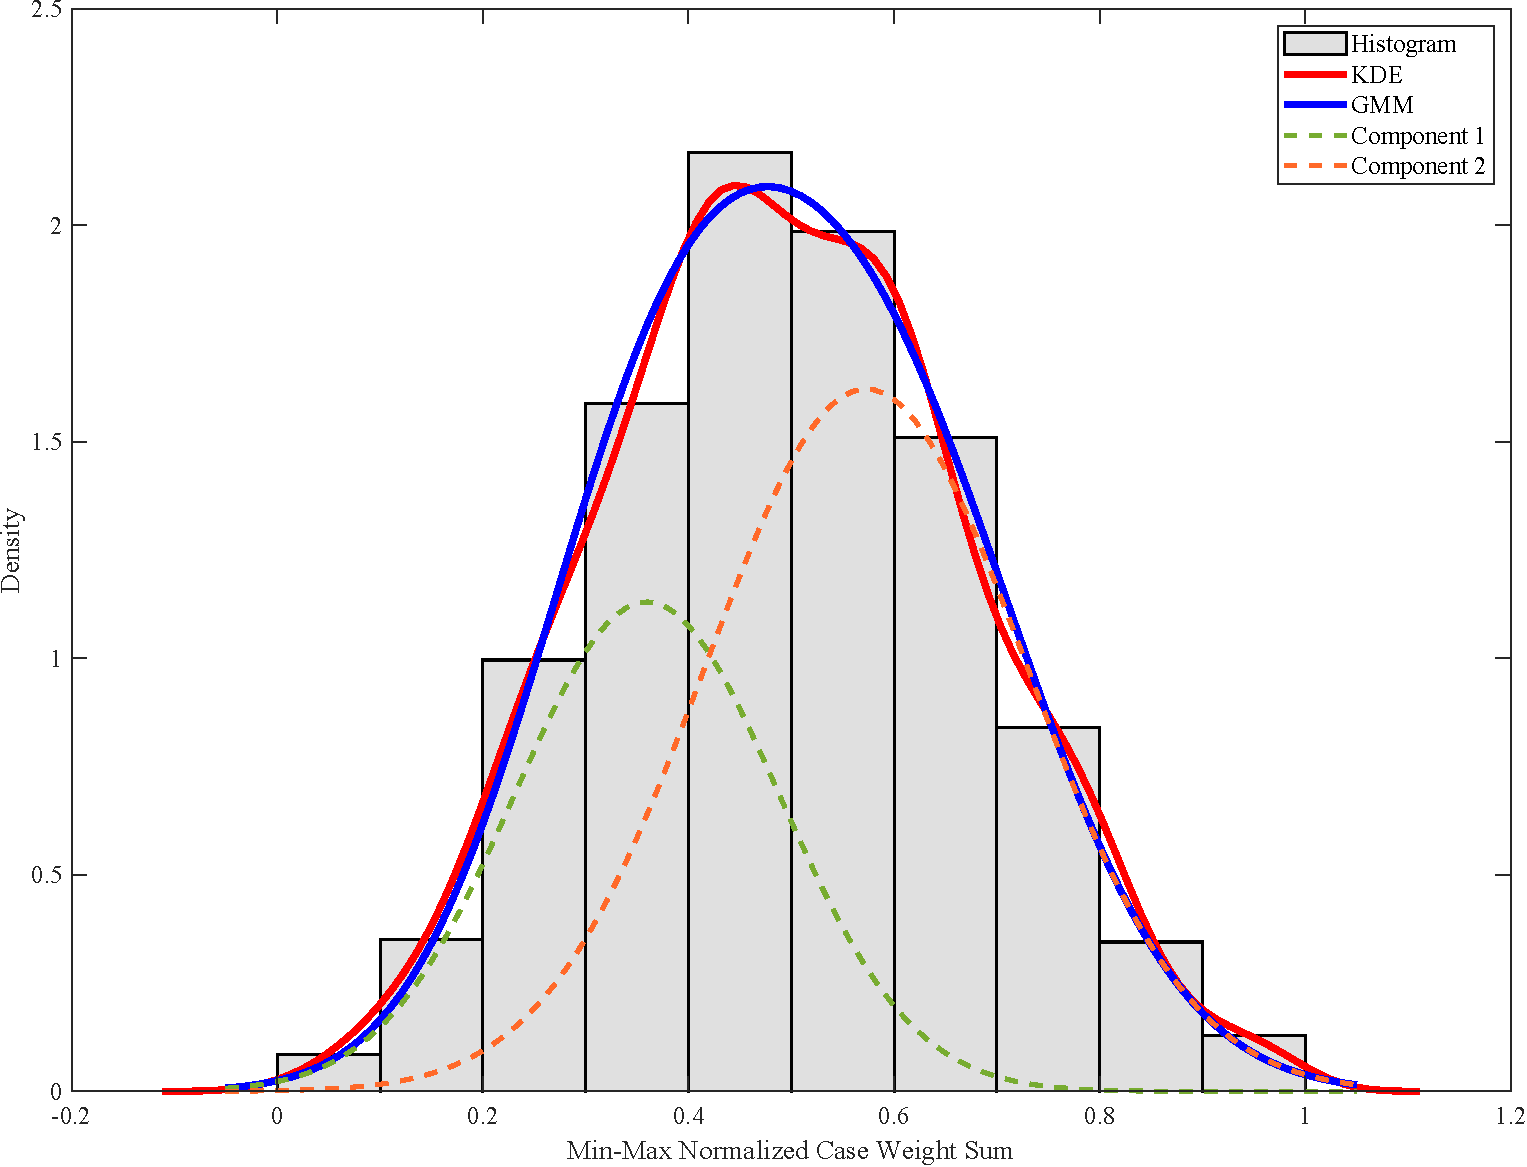
\includegraphics[width=\textwidth, keepaspectratio]{images/elicitation/approaches.pdf}
	\caption[Proposed approaches for expert opinion elicitation]{Proposed approaches for expert opinion elicitation. GMM and KDE stand for Gaussian mixture model and kernel density estimation respectively.}
	\label{fig:elicitation_approaches}
\end{figure}

\subsubsection{Posterior Probability of a Case Belonging to the Ill Subpopulation of GMM}
\label{sec:posterior-approach}
The first and second components of our GMM are shown in Figure \ref{fig:elicitation_approaches} with green and orange dotted lines respectively. If we assume that the second component represents the ill subpopulation then the posterior probability of a normalized case weight sum belonging to the second component \cite{Reynolds2009} can be defined as the EM probability as shown in Equation (\ref{eq:posterior}).
\begin{equation}
	\label{eq:posterior}
	p\left(\kappa_{2} \vert  x\right) = \frac{\varnothing_{2}\mathcal{N}\left(x\right\vert  \mu_{2},\sigma_{2})}{\sum_{m = 1}^{2}\varnothing_{m}\mathcal{N}\left(x\right\vert  \mu_{m},\sigma_{m})}
\end{equation}

\subsubsection{Cumulative Probability from Density Estimate Based on Kernel Density Estimation}
\label{sec:KDE-approach}
We used a Gaussian kernel with bandwidth, $h=0.03676$ on our $n_l=1,536$ data points for the probability density estimation of the normalized weight sum variable as shown in Equation (\ref{eq:KDE}).
\begin{equation}
	\label{eq:KDE}
	\hat{f}_{KDE}\left(x\right) = \frac{1}{n_l\times h}\sum_{l = 1}^{n_l}\frac{1}{2\pi }e^{-0.5\left(\frac{x-\tilde{s}_{c_{l}}}{h }\right)^{2}}
\end{equation}
The red curve in Figure \ref{fig:elicitation_approaches} shows the estimated density function. We defined the cumulative probability of a normalized case weight sum as the probability of having EM as shown in Equation (\ref{eq:KDE-prob}).
\begin{equation}
	\label{eq:KDE-prob}
	\hat{F}_{KDE}\left(x\right) =  \int_{-\infty }^{x}\hat{f}_{KDE}\left(x\right)dx
\end{equation}
\begin{figure}[htb!]
	\centering
	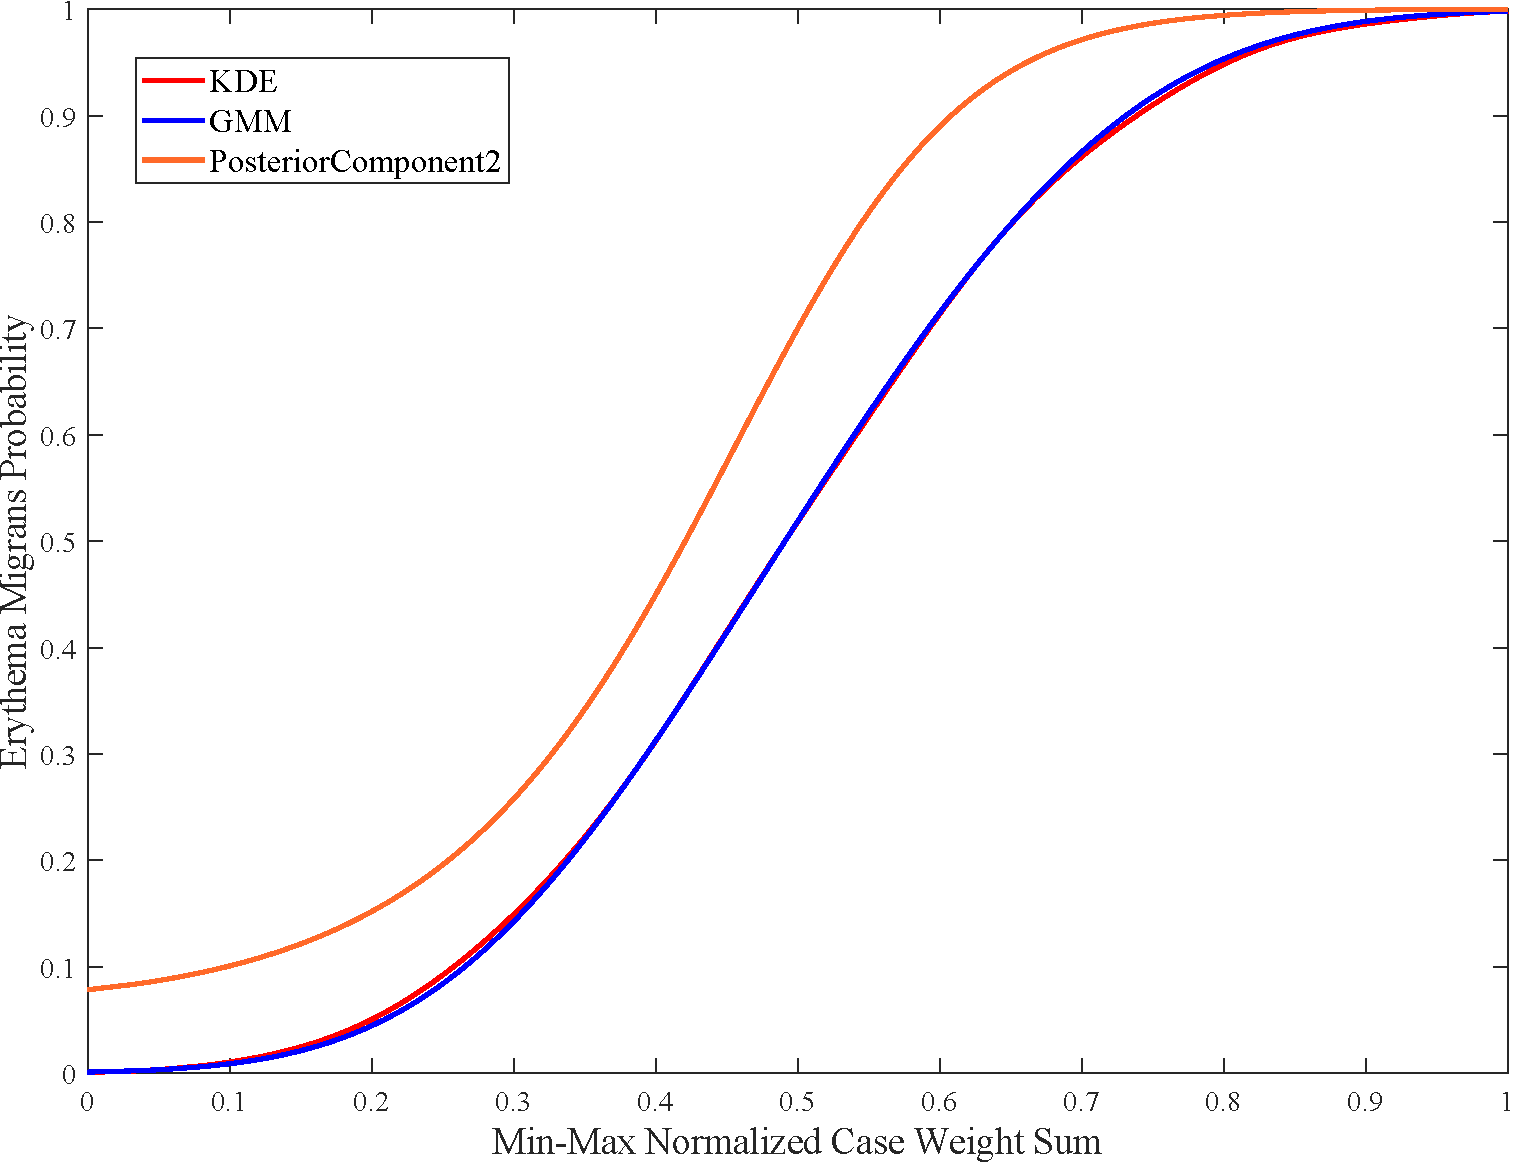
\includegraphics[width=\textwidth, keepaspectratio]{images/elicitation/probability-plot.pdf}
	\caption[Elicited erythema migrans probability plot]{Elicited erythema migrans probability plot. Blue and red lines represent the probability scores based on density estimates from Gaussian mixture model and kernel density estimate respectively. Orange line represents probability scores based on the posterior probability of a case belonging to the second component i.e. the ill subpopulation of the Gaussian mixture model.}
	\label{fig:probability_plot}
\end{figure}

\subsubsection{Elicitation Result and Analysis}
\label{sec:resanddis}
We calculated EM probability score for all possible cases using the three approaches described in Section \ref{sec:GMM-approach}, \ref{sec:posterior-approach}, and \ref{sec:KDE-approach} and presented the results with explanations to the experts in a meeting held in May 2022. Figure \ref{fig:probability_plot} shows the EM probability plot for all the cases using the three approaches. In the figure blue and red lines represent the probability scores based on density estimates from the Gaussian mixture model (approach 1) and kernel density estimate (approach 2) respectively. The orange line represents probability scores based on the posterior probability of a case belonging to the second component i.e. the ill subpopulation of the Gaussian mixture model (approach 3). Results obtained from approach 1 and approach 2 are close because both of them are based on density estimates whereas, probability scores obtained from approach 3 are always higher than the other two approaches. Based on the results and explanations the experts came to a consensus on the use of approach 1 (described in Section \ref{sec:GMM-approach}) mainly because the density estimate in approach 1 is smoother compared to approach 2 (described in Section \ref{sec:KDE-approach}).

To validate elicited model and explain its behavior to the experts first we used decision trees. For building the decision tree, we divided calculated EM probability scores into three categories: LOW (scores in the range $[0, 0.33)$), MEDIUM (scores in the range $[0.33, 0.68)$), and HIGH (scores in the range $[0.68, 1]$) Figure \ref{fig:decision_tree} shows a pruned version of the decision tree for approach 1. In the figure, each node shows the majority category along with the percentage and number of cases belonging to each category. From the tree, we can see that the model assigns HIGH EM probability to cases whenever the first answer, \enquote{\textit{yes}} to the third question \enquote{\textit{Is the size of the spot increasing or has it gradually increased}}, \( a_{1,q_{3}}\) is true. This behavior supports the doctors’ opinion because the first answer to the third question has the highest weight given by most of the doctors.
\begin{figure}[htb!]
	\centering
	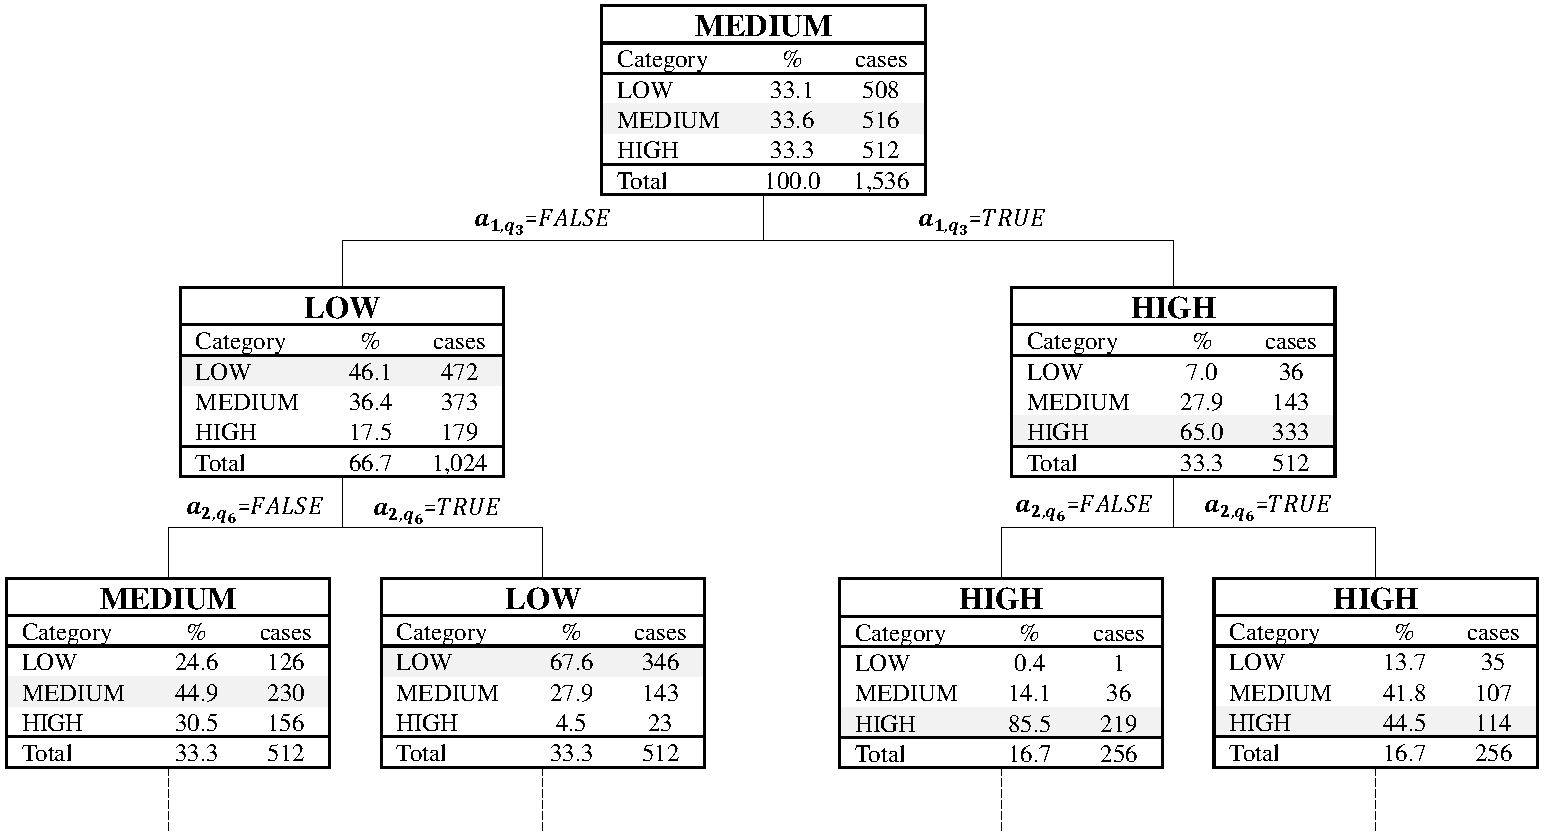
\includegraphics[width=\textwidth, keepaspectratio]{images/elicitation/decision-tree.pdf}
	\caption[Pruned decision tree explaining elicited erythema migrans probability model behavior]{Pruned decision tree explaining elicited erythema migrans probability model behavior. Each node shows the majority category along with percentage and number of cases belonging to each category. Refer to Table \ref{tab:modified_opinion} for details about the questions and answers. The full tree is available at the link stated in Appendix Section \ref{sec:app-online-elicitaion}.}
	\label{fig:decision_tree}
\end{figure}

To further explain the behavior of the model we utilized formal concept analysis (FCA) to find out questions and answers important for different probability groups. Figure \ref{fig:FCA_lattice} shows a simplified FCA lattice view for the 162 cases belonging to the lowest probability score group in the range $[0,0.1)$ obtained from approach 1.
\begin{figure}[htb!]
	\centering
	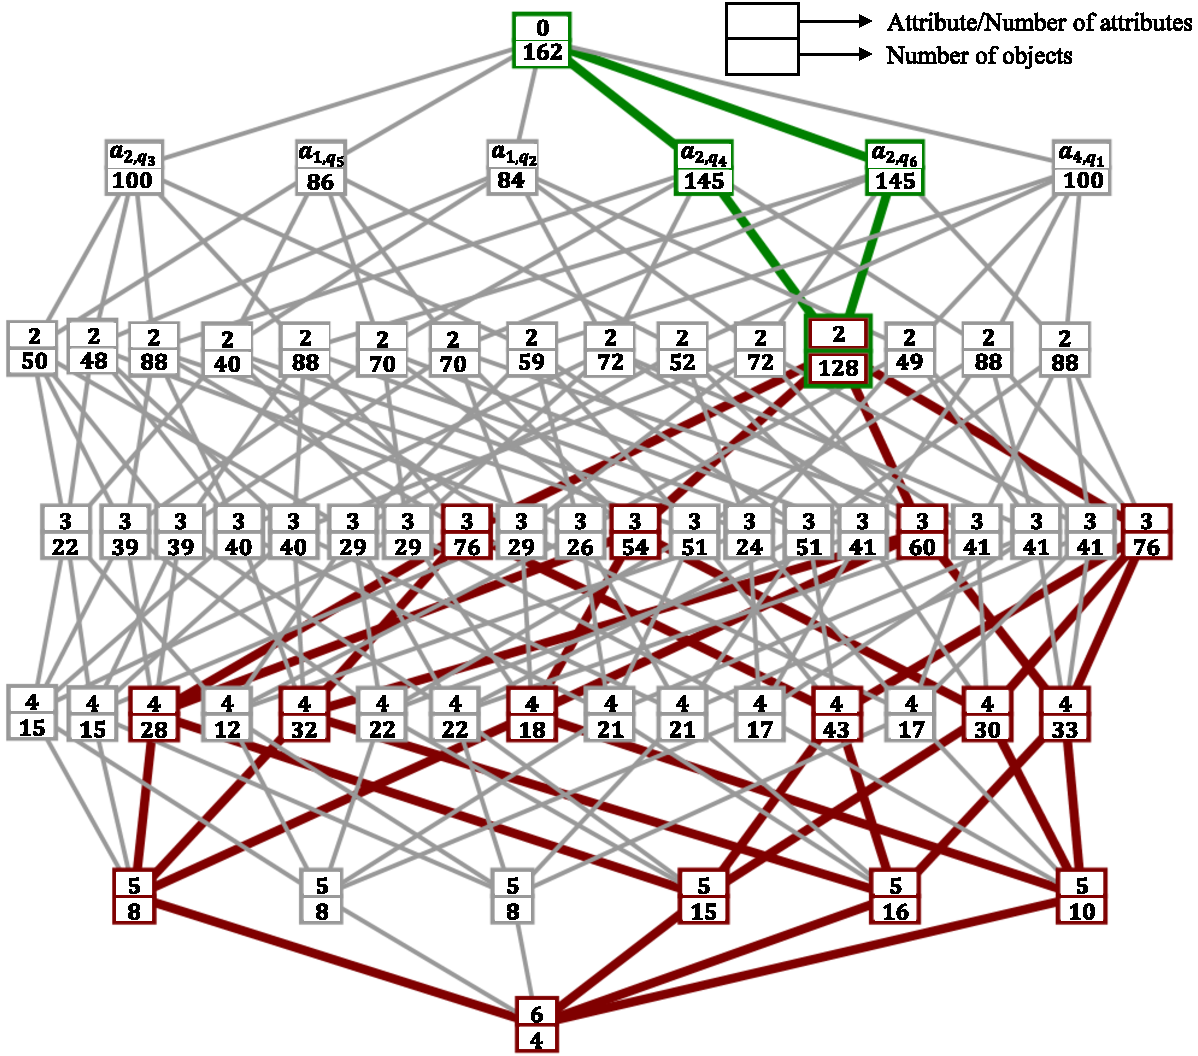
\includegraphics[width=\textwidth, keepaspectratio]{images/elicitation/FCA-lattice.pdf}
	\caption[Concept lattice view for 162 very low probability score cases in the range  $[0,0.1)$]{Concept lattice view for 162 very low probability score cases in the range  $[0,0.1)$. The top box of a node represents an attribute (answer) or a number of attributes, which are connected by lines, and the bottom box represents how many objects (cases) contain the corresponding attribute shown in the top box. Refer to Table \ref{tab:modified_opinion} for details about the questions and answers.}
	\label{fig:FCA_lattice}
\end{figure}
In the figure, the top box of a node represents an attribute (answer) or a number of attributes, which are connected by lines, and the bottom box represents how many objects (cases) contain the corresponding attribute shown in the top box. In Figure \ref{fig:FCA_lattice}, we start with 162 cases in the root node. At the first level, the number inside the bottom box of a node represents how many cases out of 162 cases contain the corresponding answer shown in the top box. For example, the \enquote{\textit{no}} answer to the question \enquote{\textit{Outdoor activities in the last 30 days before the onset of the red spot}}, \( a_{2,q_{6}}\)  is present in 145 cases. At the second level, each node represents how many cases contain two answers connected by a line. For example, \( a_{2,q_{4}}\) and \( a_{2,q_{6}}\) are jointly true in 128 cases. The rest of the FCA lattice is organized similarly. We can see from the figure that the answers common to most of these cases are the ones having lowest assigned weights or the opposites of the answers having highest assigned weights by most of the doctors.

The elicited EM probability scores for all possible cases, detailed decision tree, and FCA context files for different probability score groups are available at the link stated in Appendix Section \ref{sec:app-online-elicitaion}.

\section{Combining Probabilities from Image and Patient Data}\label{sec:combining_prob}
Our experiments showed that some images are too confusing to classify even for experts. Based on this evidence, experts suggest that EM probability obtained from the image data should not be prioritized and probability from patient data should have veto power over image data. If the EM probability obtained from image data and patient data are $p_{image}$ and $p_{data}$ respectively then the combined probability, $p_{combined}$ using the geometric mean as $\sqrt{p_{image} \times p_{data}}$ ensures veto power both for image and patient data as shown in Figure \ref{fig:gmean_normal}. But according to the experts’ suggestion, we want to keep the veto power only for the patient data. To achieve this, we made  $p_{image}$ less extreme in the lower half probability range using the transformation shown in Equation \ref{eq:less_extreme_eq}. This transformation is popular in the literature of forecast probability aggregation for making the forecasts less or more extreme \cite{baron2014two, karmarkar1978subjectively, shlomi2010subjective}. 
\begin{equation}
	\label{eq:less_extreme_eq}
	\tilde{p}_{image}=\frac{{p_{image}}^{\vartheta_{image}}}{{p_{image}}^{\vartheta_{image}}+{\left ( 1-p_{image} \right )}^{\vartheta_{image}}}
\end{equation}
The adjustment factor  $\vartheta_{image}$  was set to 0.2 so that a very low value of  $p_{image}$  does not pull down  $p_{combined}$  too much. This value was selected based on expert's suggestion to ensure that  $p_{combined}$  will be at least  $50\%$  if  $p_{data}\geq 90\%$. The adjustment of  $p_{image}$  is shown in Figure \ref{fig:less_extreme_image}. The plot of  $p_{combined}$  after the adjustment of  $p_{image}$  is shown in Figure \ref{fig:gmean_adjusted}. From the figure, we can see that the veto power was retained for  $p_{data}$  while effectively revoking it from  $p_{image}$. As geometric mean uses multiplication we replaced a zero value of  $p_{image}$  or  $p_{data}$  with a small value of 0.1 to avoid a zero value of  $p_{combined}$. 
\begin{figure}[t!]
	\centering
	\begin{subfigure}[b]{0.49\textwidth}
		\centering
		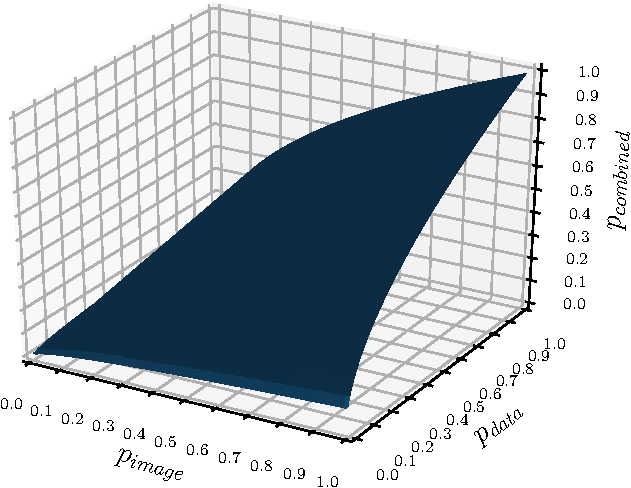
\includegraphics[width=\textwidth,keepaspectratio]{images/elicitation/combined_plot_non_extreme-cropped.pdf}
		\caption{Geometric mean.}
		\label{fig:gmean_normal}
	\end{subfigure}
	\hfill
	\begin{subfigure}[b]{0.49\textwidth}
		\centering
		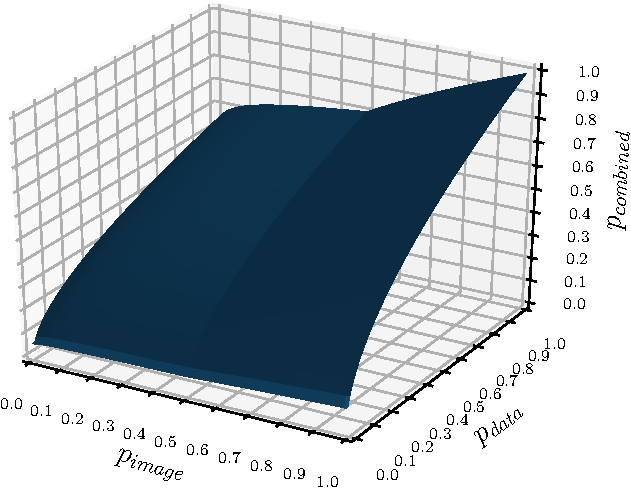
\includegraphics[width=\textwidth,keepaspectratio]{images/elicitation/combined_plot_less_extreme-cropped.pdf}
		\caption{Probability adjusted geometric mean.}
		\label{fig:gmean_adjusted}
	\end{subfigure}
	\begin{subfigure}[b]{0.75\textwidth}
		\centering
		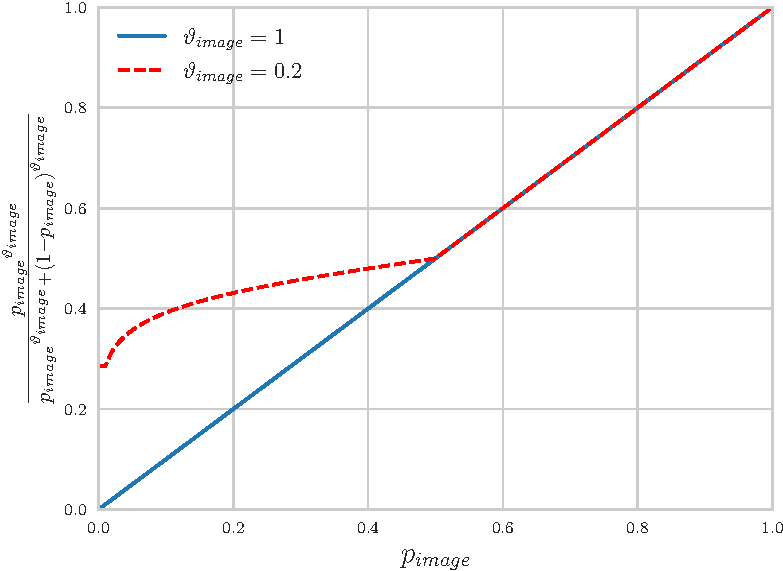
\includegraphics[width=\textwidth,keepaspectratio]{images/elicitation/less_extreme_image-cropped.pdf}
		\caption{Transformed image probability. $\vartheta_{image}$ is the transformation factor.}
		\label{fig:less_extreme_image}
	\end{subfigure}
	\caption[Combining erythema migrans probabilities from image and patient data]{Combining erythema migrans probabilities from image and patient data. $p_{image}$ and $p_{data}$ represent probabilities from image and patient data.}
	\label{fig:gmean_combination}
\end{figure}

The generalized steps involved in our strategy for combining probabilities from image and patient data are shown in Algorithm \ref{algo:combining}. The notations, inputs, and outputs are listed at the beginning of the algorithm. First, a zero value of probability from image $p_{image}$ or patient data $p_{data}$ is replaced by a small value $\epsilon$ to make sure the combined probability $p_{combined}$ does not become zero because of the geometric mean. Then, $p_{image}$ and  $p_{data}$ are transformed using the transform function. The transform function uses Equation \ref{eq:less_extreme_eq} to make the input probability less or more extreme based on the transforming factor if the input probability falls within the user-defined range. Finally, the combined probability $p_{combined}$ is calculated using the geometric mean of transformed probabilities from image $\tilde{p}_{image}$ and patient data $\tilde{p}_{data}$. Geometric mean ensures veto power for the modalities which can be adjusted using the transformation with suggestions from domain experts.
\SetKwProg{Fn}{Function}{}{}
\begin{algorithm}[]
	\DontPrintSemicolon
	\SetKwFunction{transform}{transform}
	\SetKwInOut{KwIn}{Input}
	\SetKwInOut{KwOut}{Output}
	
	\KwIn{\newline Probability estimate from lesion image: $p_{image} \in [0,1]$\newline
		Probability estimate from patient data: $p_{data} \in [0,1]$\newline
		Factor for transforming $p_{image}$: $\vartheta_{image}$\newline
		Factor for transforming $p_{data}$: $\vartheta_{data}$\newline
		Value used to avoid zero probability: $\epsilon \in (0,1]$\newline
		Range beginning for transforming $p_{image}$: $b_{image} \in [0,1]$\newline
		Range end for transforming $p_{image}$: $e_{image} \in [0,1]$\newline
		Range beginning for transforming $p_{data}$: $b_{data} \in [0,1]$\newline
		Range end for transforming $p_{data}$: $e_{data} \in [0,1]$
	}
	
	\KwOut{\newline Combined probability: $p_{combined} \in [0,1]$}
	
	% \tcc{For odd elements in the list, we add 1, and for even elements, we add 2.
		% After the loop, all elements are even.}
	% \tcp*[f]{Some thought-provoking comment.}
	% If{$\BuildOLD(a_i)$}{
		\Begin{
			\If{$p_{image}=0$}{
				$p_{image} \leftarrow \epsilon$ \tcp*[f]{avoiding zero probability from image modality}
			}    
			\If{$p_{data}=0$}{
				$p_{data} \leftarrow \epsilon$ \tcp*[f]{avoiding zero probability from patient data modality}
			}
			$\tilde{p}_{image} \leftarrow$ \transform($p_{image},\vartheta_{image}, b_{image}, e_{image}$)\tcp*[f]{transform $p_{image}$}\;
			$\tilde{p}_{data} \leftarrow$ \transform($p_{data},\vartheta_{data}, b_{data}, e_{data}$)\tcp*[f]{transform $p_{data}$}\;
			$p_{combined} \leftarrow \sqrt{\tilde{p}_{image} \times \tilde{p}_{data}}$\tcp*[f]{geometric mean}\;
			\KwRet{$p_{combined}$}
		}
		
		\Fn{transform ($p,\vartheta, b, e$)}{
			\If{$p\ge=b$ and $p\le=e$}{ 
				$p \leftarrow \frac{{p}^{\vartheta}}{{p}^{\vartheta}+{\left ( 1-p \right )}^{\vartheta}}$\tcp*[f]{transformation in specified range}
			}
			\KwRet{$p$}
		}
		\caption{Combining probabilities from image and patient data}
		\label{algo:combining}
	\end{algorithm}
	
	%(a) shows the combination using geometric mean when both the probabilities from image and patient data have veto powers. (b) shows the combination after transforming image probability to ensure veto power only for probability score from patient data. (c) shows transformation of erythema migrans probability from deep learning image classifier.
	\section{Conclusion}\label{sec:elicitation_conclusion}
	In this chapter, we successfully elicited opinions from fifteen expert doctors to create a model for obtaining EM probability score from patient data. The elicited probability model will help address the data scarcity problem towards building an effective Lyme disease pre-scanner system. We also proposed a strategy to jointly utilize EM probabilities from both image and patient data. Image-only EM analysis is not robust enough and dark skin is underrepresented in existing EM image datasets. Therefore, image-only analysis is not appropriate for a proper diagnosis of EM. We believe that combining the elicited probability score from patient data with image-based analysis can partially address these issues. The proposed techniques of questionnaire based opinion elicitation and combining probabilities from image and patient data will be useful for other diseases with similar requirements.
	
	\begin{tcolorbox}[enhanced,attach boxed title to top center={yshift=-3mm,yshifttext=-1mm},
		coltitle=black, colback=blue!5!white,colframe=blue!75!black,colbacktitle=violet!50!white,
		title=Key Points (Chapter \ref{chap:Elicitation}),fonttitle=\bfseries,
		boxed title style={colframe=black}, breakable]
		\begin{itemize}
			\item We proposed a questionnaire based expert opinion elicitation approach that utilizes Gaussian mixture model based density estimation.
			\item We opted for relative weight assignment to different answers to the questions which is easier for the experts compared to traditional approach of collecting probability estimates.
			\item We exploited decision tree and formal concept analysis for intuitive validation of the elicited model.
			\item We proposed an approach for combining the probability score from a deep learning image classifier with the elicited probability score from patient data. The proposed algorithm ensures veto power for the chosen modality based on expert's decision.
			\item For the first time, we elicited opinions from fifteen expert dermatologists to create a model for calculating erythema migrans probability from patient data as an early symptom of Lyme disease.
		\end{itemize}
	\end{tcolorbox}
